\documentclass[12pt,a4paper]{article}

% ==========================================
% 1. CÁC THƯ VIỆN CƠ BẢN VÀ ĐỊNH DẠNG
% ==========================================
\usepackage[utf8]{inputenc}
\usepackage[vietnamese]{babel}
\usepackage{geometry}
\geometry{top=2.5cm,bottom=2.5cm,left=3cm,right=2cm} % Chuẩn lề đồ án
\usepackage{amsmath, amssymb} % Toán học
\usepackage{graphicx} % Chèn ảnh
\usepackage{float} % Ép vị trí ảnh/bảng
\usepackage[table,xcdraw]{xcolor} % Màu sắc
\usepackage{tabularx, array, multirow, longtable} % Quản lý bảng biểu
\usepackage{caption, subcaption} % Quản lý chú thích ảnh
\usepackage{pbox}
\usepackage{enumitem} % Quản lý danh sách
\usepackage{tikz}
\usetikzlibrary{calc}
\usepackage{pgfplots}
\pgfplotsset{compat=1.18}
\usepackage{titlesec}
\usepackage{fancyhdr}
\usepackage{tocloft}
\usepackage{listings} % Thư viện chèn code
\usepackage{hyperref} % Tạo link mục lục có thể click
\usepackage{float}

% ==========================================
% 2. CẤU HÌNH TÙY CHỈNH (HÌNH, BẢNG, MỤC LỤC, CODE)
% ==========================================
\renewcommand{\tablename}{Bảng}
\renewcommand{\figurename}{Hình}
\renewcommand{\refname}{Tài liệu tham khảo} % Đổi tên mặc định thành tiếng Việt

% Cấu hình mục lục
\renewcommand{\cftsecaftersnum}{.}
\setlength{\cftsecnumwidth}{0.5cm}
\renewcommand{\cftsubsecaftersnum}{.}
\setlength{\cftsubsecnumwidth}{0.8cm}
\renewcommand{\cftsubsubsecaftersnum}{.}
\setlength{\cftsubsubsecnumwidth}{1.2cm}

% Cấu hình hiển thị Code
\lstset{
    backgroundcolor=\color{lightgray!20},   
    basicstyle=\ttfamily\small,
    breaklines=true,
    keywordstyle=\color{blue},
    stringstyle=\color{red},
    commentstyle=\color{green!60!black},
    numbers=left,
    stepnumber=1,
    tabsize=4,
    showstringspaces=false
}

% Cấu hình tiêu đề các mục
\titleformat{\section}{\normalfont\Large\bfseries}{\thesection.}{0.3cm}{}
\titleformat{\subsection}{\normalfont\large\bfseries}{\thesubsection.}{0.3cm}{}
\titleformat{\subsubsection}{\normalfont\normalsize\bfseries}{\thesubsubsection.}{0.3cm}{}
\titleformat{\paragraph}{\normalfont\normalsize\bfseries}{\theparagraph.}{0.3cm}{}
\titleformat{\subparagraph}{\normalfont\normalsize\bfseries}{\thesubparagraph.}{0.5em}{}
\titlespacing*{\subparagraph}{0pt}{3.25ex plus 1ex minus .2ex}{1.5ex}

% Cấu hình Header và Footer
\pagestyle{fancy}
\fancyhf{}
\renewcommand{\headrulewidth}{0.3pt}
\fancyhead[L]{\textit{UET-FET}}
\fancyhead[C]{\textit{SPRING 2026}}
\fancyhead[R]{\textit{ELT3102\_16}}
\fancyfoot[C]{\thepage}
\fancypagestyle{plain}{
    \fancyhf{}
    \fancyfoot[C]{\thepage}
    \renewcommand{\headrulewidth}{0pt}
}

% ==========================================
% 3. BẮT ĐẦU TÀI LIỆU
% ==========================================
\begin{document}

\begin{titlepage}
% -------- KHUNG BÌA --------
\begin{tikzpicture}[remember picture,overlay]
\draw[line width=1.5pt]
    ($(current page.north west)+(1.3cm,-1.3cm)$)
    rectangle
    ($(current page.south east)+(-1.3cm,1.3cm)$);
\draw[line width=0.8pt]
    ($(current page.north west)+(1.4cm,-1.4cm)$)
    rectangle
    ($(current page.south east)+(-1.4cm,1.4cm)$);
\end{tikzpicture}

\centering
\textbf{\Large ĐẠI HỌC QUỐC GIA HÀ NỘI}\par
\vspace{0.3cm}
\textbf{\Large TRƯỜNG ĐẠI HỌC CÔNG NGHỆ}\par

\vfill

\includegraphics[width=6cm]{uetlogo} 
\vfill

\textbf{\huge BÁO CÁO DỰ ÁN}\\[0.8cm]
\textbf{\Large Trạm Xử Lý Âm Thanh} \\[0.5cm] 

\vfill

% --- PHẦN THÔNG TIN ---
\begin{minipage}{\textwidth}
    \centering
    \large 
    \textbf{Học phần:} Xử lý tín hiệu số \\
    \textbf{Mã học phần:} ELT3144\_6 \\
    \textbf{Sinh viên:} Trần Thái Huy \\
    \textbf{MSSV:} 24021830 \\
    \textbf{Giảng viên:} Trần Thị Thúy Quỳnh \\
\end{minipage}

\vfill
\textbf{Hà Nội, 2026}
\end{titlepage}

\newpage
\pagestyle{plain} 
\tableofcontents % Tạo mục lục tự động
\newpage
\pagestyle{fancy} % Bật lại header/footer cho các trang nội dung

% ==========================================
% NỘI DUNG BÁO CÁO
% ==========================================

\section{Giới thiệu tổng quan}
Trạm xử lý âm thanh là hệ thống sử dụng công cụ MATLAB nhằm thực hiện quá trình lọc số và xử lý các tín hiệu âm thanh (audio) theo thời gian thực. Hệ thống yêu cầu sự kết hợp chặt chẽ giữa các thuật toán xử lý tín hiệu số và công cụ MATLAB App Designer, tính năng được tích hợp sẵn từ các phiên bản MATLAB 2014b trở về sau, dựa trên nghiên cứu tại 
\cite{ref_dafx} \cite{ref_NLT}.
\subsection{Mục tiêu đề tài}
\begin{itemize}[label=$\bullet$]
    \item \textbf{Về lý thuyết:} Áp dụng các kiến thức cốt lõi của môn Xử lý tín hiệu số (như thuật toán phân tích phổ FFT/DFT, thiết kế bộ lọc số IIR/FIR, và đặc tuyến bộ lọc Butterworth) vào bài toán thực tế. Đồng thời, kết hợp và vận dụng linh hoạt các bộ công cụ trên môi trường lập trình MATLAB. 
    \item \textbf{Về thuât toán:} Xây dựng thành công hệ thống phân tách tín hiệu âm thanh thành các dải tần số riêng biệt mà vẫn đảm bảo độ trung thực, không làm méo dạng tín hiệu gốc.
    \item \textbf{Về phần mềm:} Thiết kế giao diện người dùng (GUI) trực quan và thân thiện thông qua nền tảng MATLAB App Designer. Ứng dụng cho phép người dùng nạp các tệp âm thanh (định dạng .wav hoặc .mp3) và tùy chỉnh hệ số khuếch đại (Gain) cho từng dải tần số một cách tương tác. 
    \item \textbf{Về giới hạn phạm vi:} Hệ thống tập trung xử lý luồng dữ liệu âm thanh ngoại tuyến (đọc từ các tệp lưu trữ có sẵn) thay vì thu thập và xử lý tín hiệu trực tiếp từ micro.
\end{itemize}

\section{Cơ sở lý thuyết và tính toán}

\subsection{Số hóa tín hiệu âm thanh và Định lý Nyquist}
Quá trình chuyển đổi tín hiệu tương tự sang tín hiệu số (quá trình số hóa) gồm ba bước cơ bản được thực hiện theo thứ tự: Lấy mẫu (sampling), lượng tử hóa (quantization) và mã hóa (coding). Bước lấy mẫu là quá trình rời rạc hóa tín hiệu liên tục $x(t)$ thành chuỗi tín hiệu $x(nT)$ thông qua việc nhân với chuỗi xung Dirac theo chu kỳ $T$. Quá trình này bắt buộc phải tuân theo định lý lấy mẫu Nyquist-Shannon: Để có thể khôi phục lại tín hiệu gốc mà không bị mất mát thông tin, tần số lấy mẫu $f_s$ phải lớn hơn ít nhất hai lần tần số cực đại $f_{max}$ có trong tín hiệu:
\begin{equation}
    f_s \geq 2f_{max}
\end{equation}

Tần số Nyquist được định nghĩa là $f_n = f_s/2$. Thông qua phân tích phổ bằng biến đổi Fourier, có thể chứng minh được rằng nếu tín hiệu đầu vào chứa các thành phần tần số vượt qua mốc $f_n$ này, hiện tượng chồng phổ (aliasing) sẽ lập tức xảy ra, làm sai lệch hoàn toàn dữ liệu âm thanh số.

Đối với các hệ thống xử lý tín hiệu âm thanh, tỷ số tín hiệu trên nhiễu lượng tử (SQNR) là một thông số cực kỳ quan trọng đối với bộ chuyển đổi tương tự - số (ADC). Mức SQNR lý tưởng được tính theo số bit $n$ của bộ chuyển đổi như trong phương trình \ref{eq:sqnr}:
\begin{equation} \label{eq:sqnr}
    SQNR = 1.76 + 6.02n \quad \text{(dB)}
\end{equation}

\subsection{Tổng quan về Bộ lọc số: IIR và FIR}
Bộ lọc số trong Xử lý tín hiệu được chia làm hai họ chính:
\begin{itemize}
    \item \textbf{FIR (Finite Impulse Response):} Là bộ lọc có đáp ứng xung hữu hạn. Hàm truyền của bộ lọc FIR có dạng tổng quát:
    \begin{equation}
        H(z) = b_0 + b_1 z^{-1} + b_2 z^{-2} + \dots + b_N z^{-N} = \sum_{n=0}^{N} b_n z^{-n}
    \end{equation}
    Ưu điểm của FIR là luôn ổn định và có thể thiết kế để đạt được pha tuyến tính, không làm méo pha của tín hiệu âm thanh. Tuy nhiên, để đạt được độ dốc cắt tần (roll-off) cao, bộ lọc FIR đòi hỏi bậc $N$ rất lớn, gây tiêu tốn tài nguyên bộ nhớ và tạo ra độ trễ (delay) trong tính toán.
    
    \item \textbf{IIR (Infinite Impulse Response):} Là bộ lọc có đáp ứng xung vô hạn, sử dụng cấu trúc có phản hồi (feedback). Hàm truyền của bộ lọc IIR có dạng một phân thức hữu tỉ:
    \begin{equation}
        H(z) = \frac{\sum_{i=0}^{M} b_i z^{-i}}{1 + \sum_{j=1}^{N} a_j z^{-j}} = \frac{b_0 + b_1 z^{-1} + \dots + b_M z^{-M}}{1 + a_1 z^{-1} + \dots + a_N z^{-N}}
    \end{equation}
    Trong đó, $b_i$ là các hệ số truyền thẳng (feedforward) và $a_j$ là các hệ số phản hồi (feedback). Chính nhờ sự xuất hiện của các hệ số phản hồi $a_j$ ở mẫu số, IIR chỉ cần bậc rất thấp để đạt được đáp ứng biên độ (độ dốc cắt tần) tương đương với bộ lọc FIR bậc cao. Điều này làm giảm đáng kể khối lượng tính toán và độ trễ, cực kỳ phù hợp cho các trạm xử lý âm thanh theo thời gian thực (như hệ thống Equalizer).
\end{itemize}
\subsection{Các loại đáp ứng dải tần (Lowpass, Highpass, Bandpass)}
Trong ứng dụng Equalizer, tín hiệu âm thanh tổng hợp được phân tách thành các dải tần riêng biệt thông qua các cấu hình đáp ứng lọc cơ bản:
\begin{itemize}
    \item \textbf{Lowpass (Lọc thông thấp):} Chỉ cho phép các tín hiệu có tần số thấp hơn tần số cắt $f_c$ đi qua, loại bỏ tần số cao.
    \item \textbf{Highpass (Lọc thông cao):} Chỉ cho phép các tín hiệu có tần số cao hơn $f_c$ đi qua, loại bỏ tần số thấp.
    \item \textbf{Bandpass (Lọc thông dải):} Là sự kết hợp của Lowpass và Highpass, chỉ cho phép tín hiệu nằm trong khoảng dải thông từ $f_{c1}$ đến $f_{c2}$ đi qua. Trong hệ thống này, Bandpass được sử dụng làm thành phần chủ đạo để cô lập 5 dải tần: Bass, Low-Mid, Mid, High-Mid và Treble.
\end{itemize}

\subsection{Các họ bộ lọc}
Về mặt lý thuyết, một bộ lọc lý tưởng (ideal filter) |H(omega)| không làm méo biên độ của phổ và phi(omega) không làm méo pha của phổ tín hiệu đầu vào X(omega). Khi đầu vào x(t) đi qua một bộ lọc lý tưởng thì đầu ra có dạng: y(t) = kx(t-T0) với T0 là một quá trị thời gian làm trễ. Tuy nhiên, theo định lý Paley-Wiener, một bộ lọc lý tưởng như vậy đòi hỏi đáp ứng xung trong miền thời gian là một hàm \textit{sinc} kéo dài vô hạn từ $-\infty$ đến $+\infty$. Tuy nhiên trong thực tế không có tín hiệu vô hạn. 
Vì vậy, trong thực tế, mọi thiết kế bộ lọc đều là các phép gần đúng và buộc phải chấp nhận sự tồn tại của dải chuyển tiếp (transition band), cũng như hiện tượng nhấp nhô (ripple) ở dải thông hoặc dải chắn. 

\vspace{0.5cm} 
\noindent\textbf{Họ bộ lọc Butterworth:} Đặc trưng nổi bật nhất của họ bộ lọc Butterworth là tính chất "phẳng tối đa" (maximally flat) trong dải thông. Loại bộ lọc này có $A^2(-s^2)$ được xấp xỉ bởi:
\begin{equation} \label{eq:butterworth}
    A^2(\Omega) = \frac{1}{1 + \left(\frac{\Omega}{\Omega_c}\right)^{2n}}
\end{equation}

Trong đó:
\begin{itemize}[label=--]
    \item $n$: Bậc của bộ lọc.
    \item $\Omega_c$: Tần số cắt của bộ lọc (rad/s).
    \item $\Omega$: Tần số góc của tín hiệu đầu vào (rad/s).
\end{itemize}

Từ Phương trình \ref{eq:butterworth}, ta có thể thấy tại vị trí tần số cắt ($\Omega = \Omega_c$), biên độ tín hiệu luôn thỏa mãn $A^2(\Omega_c) = 1/2$. Điều này có nghĩa là đáp ứng biên độ tại điểm cắt luôn bị suy giảm chính xác $3 \text{ dB}$ (tương đương mức điện áp giảm còn $\approx 0.707$ lần), bất kể bộ lọc được thiết kế ở bậc $n$ bằng bao nhiêu.

Hình \ref{fig:butterworth_response} mô tả $A^2(-s^2)$ và đáp ứng tần số biên độ hệ thống $|H(\Omega)|$ tương ứng cho bộ lọc Butterworth với các bậc khác nhau.

\begin{figure}[H]
    \centering
    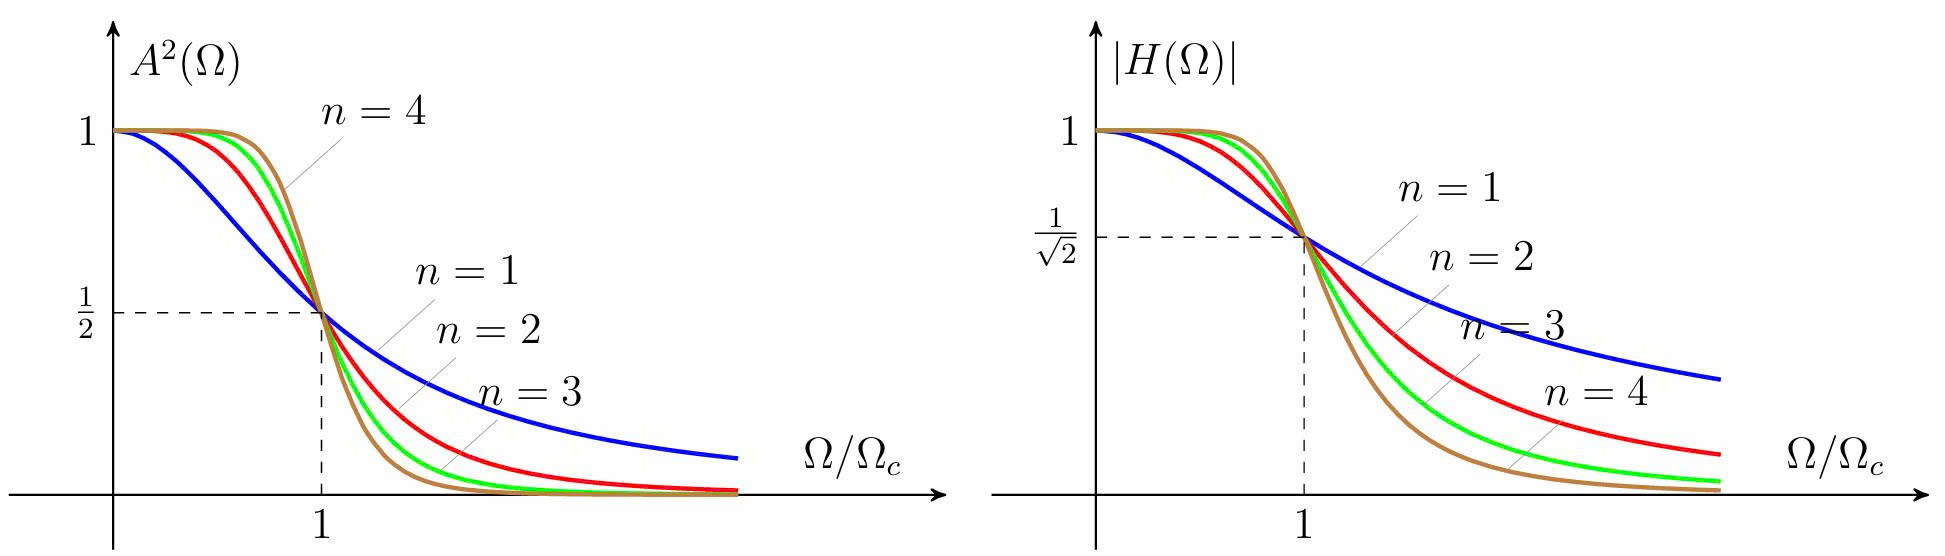
\includegraphics[width=0.7\textwidth]{butterworth.jpg}
    \caption{Đáp ứng tần số của bộ lọc Butterworth với các bậc $n$ khác nhau có cùng tần số cắt chuẩn hóa $\Omega_c = 1 \text{ rad/s}$}
    \label{fig:butterworth_response}
\end{figure}

\vspace{0.5cm} 
\noindent\textbf{Họ bộ lọc Chebyshev (Chebychev):} Đối với họ bộ lọc này, đáp ứng có độ gợn sóng đều (ripple) trong dải thông. Thuật toán thiết kế sử dụng xấp xỉ toán học dựa trên họ các đa thức Chebyshev bậc $n$, được định nghĩa theo hệ phương trình hàm piecewise sau:
\begin{equation}
    C_n(x) = 
    \begin{cases} 
        \cos(n \cdot \arccos(x)), & |x| \leq 1 \\
        \cosh(n \cdot \mathrm{arccosh}(x)), & |x| > 1
    \end{cases}
\end{equation}

$C_n(x)$ là họ các đa thức trực giao trên khoảng $(-1,1)$, có giá trị cực đại là $1$ và giá trị cực tiểu là $-1$. $A^2(-s^2)$ xấp xỉ: 
\begin{equation}
    A^2(\Omega) = \frac{\alpha}{1 + \epsilon^2 C_n^2 \left( \frac{\Omega}{\Omega_c} \right)}
\end{equation}

Trong đó:
\begin{itemize}[label=--]
    \item $\epsilon$: Được lựa chọn để quy định mức độ gợn sóng cho phép trong dải thông.
    \item $\alpha$: Hệ số chuẩn hóa được xác định để thỏa mãn yêu cầu về độ tăng ích (độ khuếch đại) đối với thành phần tín hiệu một chiều (DC gain, tại tần số $\Omega = 0$).
\end{itemize}

\begin{figure}[H]
    \centering
    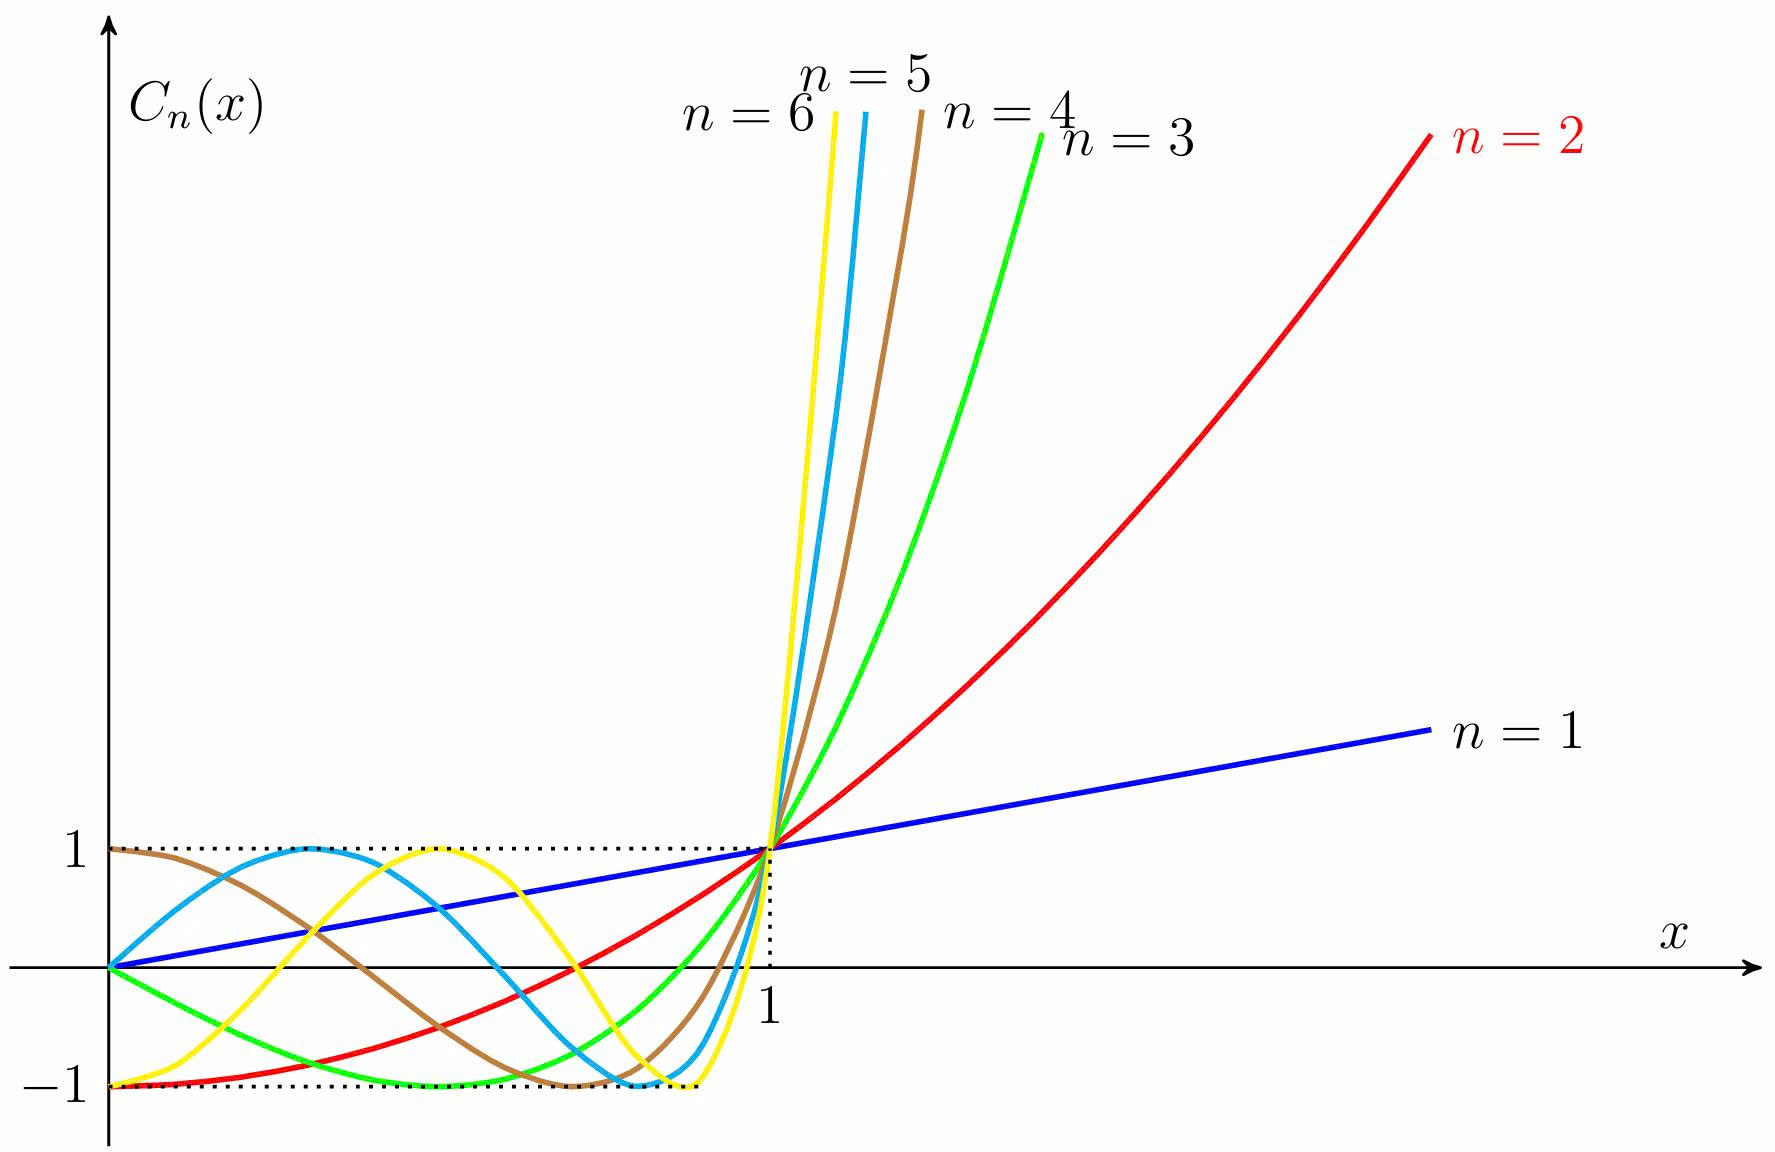
\includegraphics[width=0.7\textwidth]{chebychev.jpg}
    \caption{Gợn sóng dải triệt của các đa thức Chebychev}
    \label{fig:chebychev_response}
\end{figure}

\section{Triển khai hệ thống}
\subsection{Sơ đồ khối tổng quát}
Hệ thống Trạm xử lý âm thanh được thiết kế và vận hành hoàn toàn trên môi trường MATLAB với luồng xử lý tín hiệu tuân theo sơ đồ khối tại Hình \ref{fig:block_diagram} minh họa luồng đi của tín hiệu từ khối đầu vào cho đến khối xuất tín hiệu. Ban đầu, tín hiệu âm thanh đầu vào (định dạng .wav hoặc .mp3) được trích xuất và chuyển đổi sang tín hiệu dạng mono để đồng bộ hóa kênh xử lý. Sau đó, tín hiệu gốc được phân nhánh và đưa song song qua 5 khâu lọc thông dải (Bandpass Filter) để cô lập các dải tần số đặc trưng. 

Tại tầng phối trộn (Mixer), mỗi luồng tín hiệu dải tần được nhân với một hệ số khuếch đại (Gain) độc lập được cung cấp từ giao diện người dùng. Các luồng này sau đó được cộng gộp lại và đi qua khâu chuẩn hóa biên độ (Normalization) để triệt tiêu hiện tượng xén ngọn (clipping) trước khi đưa ra thiết bị phát (Loa) và xuất lên đồ thị phân tích phổ thời gian thực(FFT).

\begin{figure}[H]
    \centering
    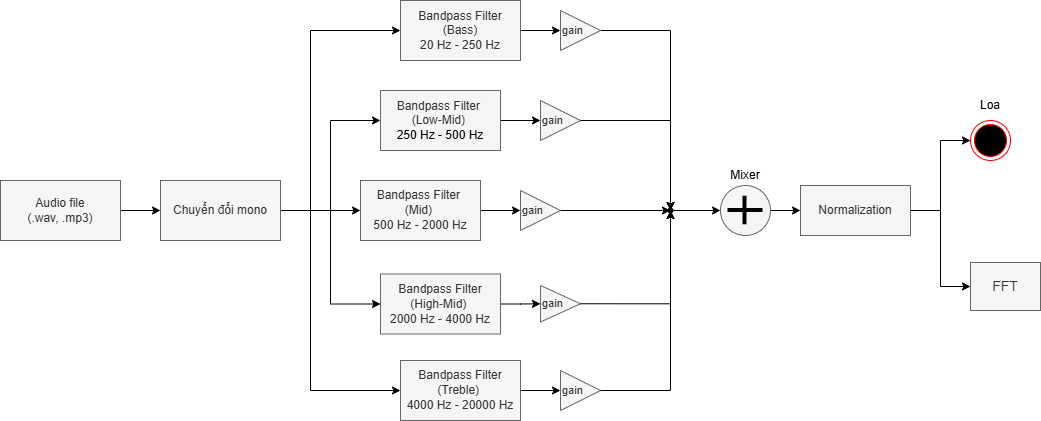
\includegraphics[width=0.8\textwidth]{so do khoi.png}
    \caption{Sơ đồ khối hệ thống }
    \label{fig:block_diagram}
\end{figure}
\subsection{Thông số các dải tần}
Dựa trên giới hạn thính giác của con người và tính âm sắc của các loại nhạc cụ, phổ tần số âm thanh (từ $20 \text{ Hz}$ đến $20 \text{ kHz}$) được phân thành 5 dải thông chính. Hệ thống sử dụng họ bộ lọc IIR Butterworth bậc $n = 4$ để thiết kế các khâu lọc thông dải. Thông số tần số cắt (Cut-off frequency) cho từng dải thông được quy định trong Bảng \ref{tab:freq_bands}.
\begin{table}[H]
    \centering
    \begin{tabular}{|c|l|c|c|}
        \hline
        \textbf{STT} & \textbf{Dải tần số (Band)} & \textbf{Tần số cắt dưới ($f_{low}$)} & \textbf{Tần số cắt trên ($f_{high}$)} \\
        \hline
        1 & Bass (Âm trầm) & $20 \text{ Hz}$ & $250 \text{ Hz}$ \\
        \hline
        2 & Low-Mid (Âm trung trầm) & $250 \text{ Hz}$ & $500 \text{ Hz}$ \\
        \hline
        3 & Mid (Âm trung) & $500 \text{ Hz}$ & $2000 \text{ Hz}$ \\
        \hline
        4 & High-Mid (Âm trung cao) & $2000 \text{ Hz}$ & $4000 \text{ Hz}$ \\
        \hline
        5 & Treble (Âm cao) & $4000 \text{ Hz}$ & $20000 \text{ Hz}$ \\
        \hline
    \end{tabular}
    \caption{Bảng quy định thông số tần số cắt cho 5 dải thông}
    \label{tab:freq_bands}
\end{table}

\subsection{Triển khai thuật toán trên MATLAB}
\noindent\textbf{Tiền xử lý tín hiệu:} Đầu vào của hệ thống là các tệp âm thanh có định dạng \texttt{.wav} hoặc \texttt{.mp3}. Sau khi trích xuất chuỗi dữ liệu biên độ mẫu ($x$) và tần số lấy mẫu ($f_s$) thông qua hàm \texttt{audioread}, hệ thống sẽ tiến hành kiểm tra số lượng kênh tín hiệu. Do hầu hết các bản nhạc trên thị trường hiện nay đều được phát hành ở định dạng âm thanh nổi (Stereo) bao gồm hai kênh trái và phải độc lập, hệ thống sẽ thực hiện quá trình chuyển đổi tín hiệu về dạng đơn kênh (Mono) bằng phương pháp tính trung bình cộng biên độ của hai kênh. Phép biến đổi này không chỉ giúp giảm thiểu 50\% khối lượng tính toán cho toàn bộ hệ thống khâu lọc phía sau, mà còn quy chuẩn dữ liệu về dạng vector một chiều (1D). Quá trình này tạo tiền đề bắt buộc để các thuật toán phân tích phổ FFT và bộ lọc IIR hoạt động ổn định và chính xác.\\
\\
\textbf{Chuẩn hóa tần số và sinh hệ số lọc:} 
Trước khi thiết kế bộ lọc, toàn bộ các điểm tần số cắt đều được chuẩn hóa theo tần số Nyquist của hệ thống ($f_n = f_s / 2$, với $f_s$ là tần số lấy mẫu của tệp âm thanh). Quá trình tìm các điểm Zero, Pole và Gain cho mỗi dải tần được thực hiện thông qua hàm \texttt{butter} tích hợp sẵn trong MATLAB:
\begin{verbatim}
    [z, p, G] = butter(n, [f_low/fn, f_high/fn], 'bandpass');
\end{verbatim}

\noindent\textbf{Phương pháp lọc tín hiệu:}
Hệ thống sử dụng họ bộ lọc IIR Butterworth bậc 4. Tuy nhiên, để đảm bảo tính ổn định tuyệt đối của hệ thống số học và triệt tiêu sai số lượng tử hóa (quantization error) khi tính toán các hệ số, hàm truyền tổng quát được phân rã thành các khâu bậc 2 ghép nối tiếp (cấu trúc Second-Order Sections - SOS) thông qua lệnh \texttt{zp2sos}. Ngoài ra, hàm \texttt{filtfilt} được sử dụng để thực hiện quá trình lọc tín hiệu hai chiều (một lần theo chiều tiến và một lần lật ngược theo chiều lùi thời gian). Cơ chế đặc biệt này giúp triệt tiêu hoàn toàn hiện tượng méo pha (phase distortion) của họ bộ lọc IIR, trong khi hệ thống vẫn tận dụng tối đa được ưu điểm cắt tần dốc và tính chất tiết kiệm tài nguyên của cấu trúc phản hồi.

\begin{verbatim}
    [b, g] = zp2sos(z, p, G);
    x_band = filtfilt(b, g, x);
\end{verbatim}

\noindent\textbf{Phối trộn (Mixer) và Chuẩn hóa (Normalization):}
Tín hiệu đầu ra ($x_{out}$) được tính toán dựa trên nguyên lý xếp chồng tuyến tính (linear superposition). Cụ thể, các luồng tín hiệu dải tần độc lập sẽ được nhân với hệ số khuếch đại (Gain) tương ứng từ thanh trượt và cộng gộp lại. Tuy nhiên, quá trình cộng dồn năng lượng này có thể làm biên độ tín hiệu tổng vượt qua giới hạn biểu diễn động của kỹ thuật số ($|x_{out}| > 1.0$), dẫn đến hiện tượng rè loa. Để khắc phục triệt để vấn đề này, hệ thống tự động thực hiện khâu chuẩn hóa biên độ (Normalization) bằng cách chia tỷ lệ toàn bộ mảng dữ liệu đầu ra cho giá trị đỉnh tuyệt đối (absolute peak) của chính nó. Thuật toán này đóng vai trò như một bộ giới hạn (Limiter) cứng, ép tín hiệu luôn nằm trong ngưỡng an toàn $[-1.0, 1.0]$:
\begin{verbatim}
    x_out = (gain_bass * x_bass) + ... + (gain_treble * x_treble);
    x_out = x_out / max(abs(x_out));
\end{verbatim}

\subsection{Đặc tuyến đáp ứng của các bộ lọc}

\begin{figure}[H]
    \centering
    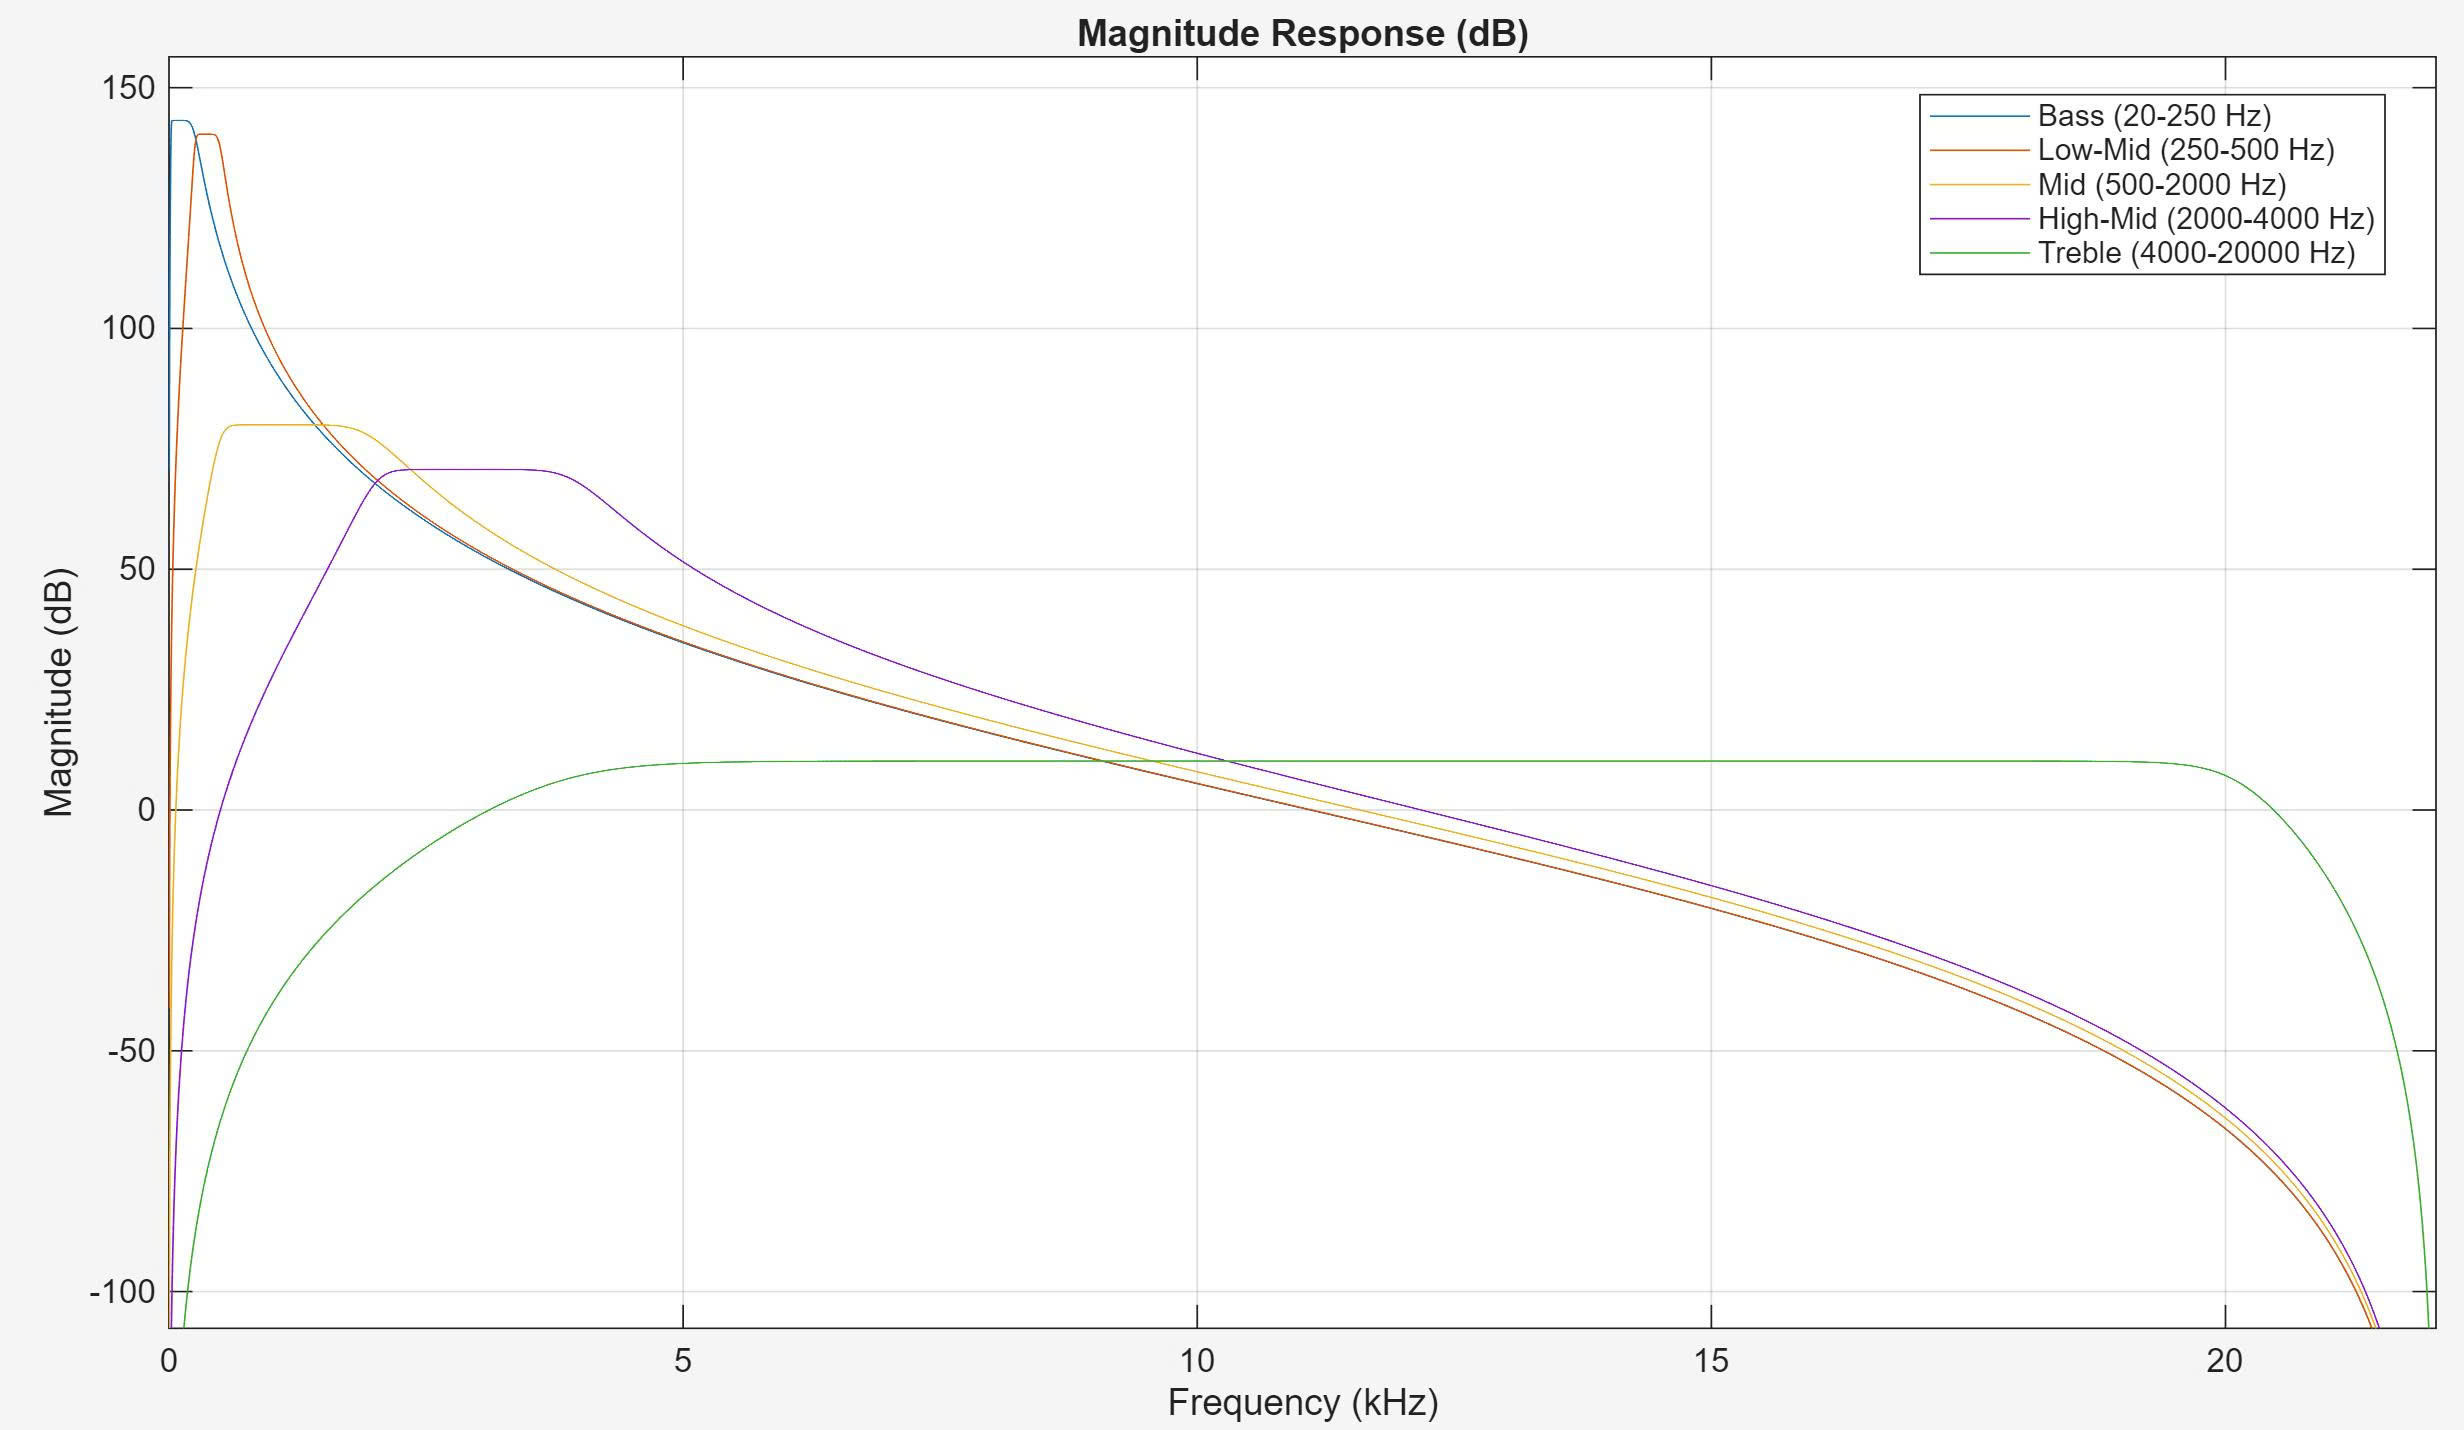
\includegraphics[width=0.85\textwidth]{magnitude_response.jpg}
    \caption{Đáp ứng biên độ (Magnitude Response).}
    \label{fig:magnitude_response}
\end{figure}

Hình \ref{fig:magnitude_response} mô tả đặc tuyến đáp ứng biên độ của 5 dải thông sau khi được tính toán và thiết kế bằng họ bộ lọc IIR Butterworth bậc 4. Trục hoành biểu diễn tần số theo thang đo logarit. Có thể quan sát thấy độ dốc cắt tần lý tưởng $-24 \text{ dB/octave}$ và sự giao thoa (crossover) chính xác tại điểm $-3 \text{ dB}$ giữa các băng tần kề nhau. Biểu đồ cũng cho thấy các bộ lọc đã cô lập thành công 5 dải tần số riêng biệt mà không tạo ra hiện tượng gợn sóng (ripple) trong dải thông, đúng với lý thuyết của phân bố Butterworth.

\begin{figure}[H]
    \centering
    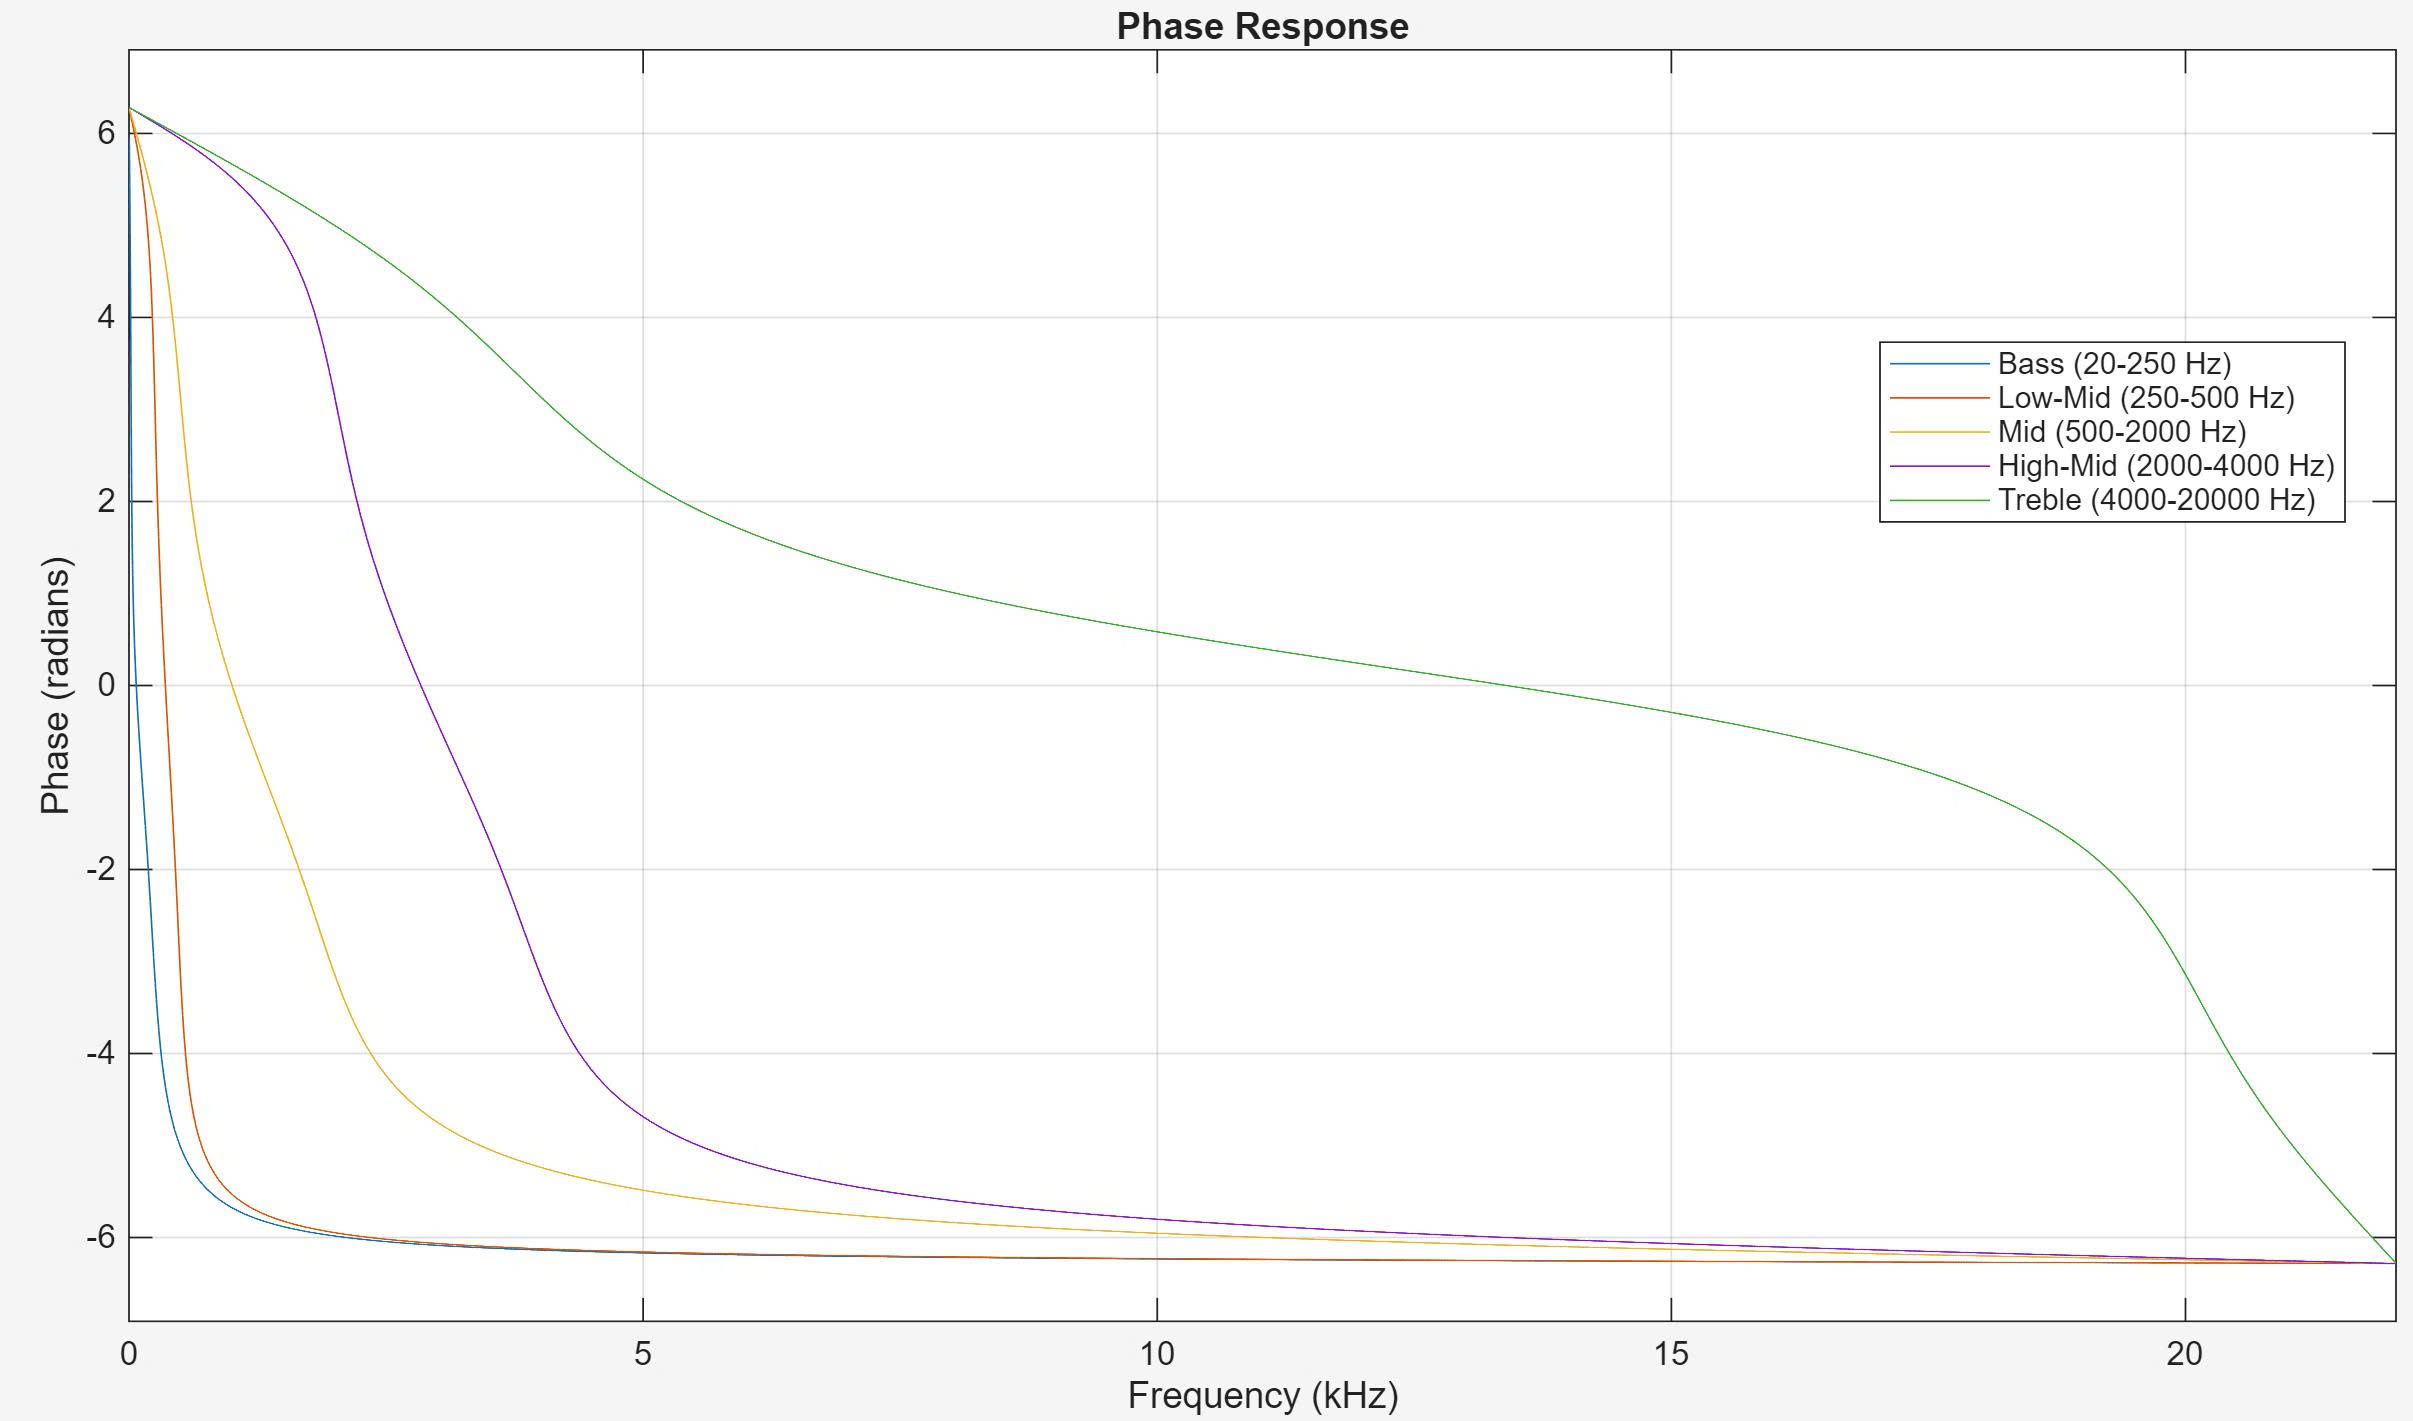
\includegraphics[width=0.7\textwidth]{phase_response.jpg}
    \caption{Đáp ứng pha (Phase Response). }
    \label{fig:phase_response}
\end{figure}
Mặc dù họ bộ lọc IIR gốc mang đặc tính pha phi tuyến, nhưng trong đồ thị ở hình \ref{fig:phase_response} lại cho thấy đáp ứng pha tổng thể đã được triệt tiêu hoàn toàn về mức 0 (zero-phase). Điều này là minh chứng rất rõ cho hiệu quả của việc ứng dụng hàm lọc hai chiều \texttt{filtfilt} ở khâu xử lý, giúp ngăn chặn tuyệt đối hiện tượng méo pha khi các giải âm thanh được phối trộn.

\subsection{Thiết kế giao diện người dùng (GUI)}
Phần mềm được thiết kế và trực quan hóa thông qua nền tảng MATLAB App Designer. Giao diện ứng dụng (Hình \ref{fig:gui_app}) được cấu trúc thành ba khối chức năng chính bao gồm:
\begin{itemize}
    \item \textbf{Khối điều khiển:} Nút bấm \texttt{Choice} cho phép người dùng lựa chọn và nạp các tệp âm thanh ngoại tuyến (định dạng \texttt{.wav} hoặc \texttt{.mp3}), từ đó tự động kích hoạt tiến trình phân tách thành 5 dải tần số. Song song với đó, cụm nút \texttt{Play/Stop} chịu trách nhiệm quản lý trực tiếp vòng đời và trạng thái hoạt động của đối tượng phát tín hiệu (\texttt{audioplayer}).
    \item \textbf{Khối tùy chỉnh:} Bao gồm 5 thanh trượt (Slider) tương ứng với 5 băng tần đã thiết kế. Mỗi khi người dùng tương tác thay đổi giá trị, hệ thống sẽ lập tức bắt sự kiện \texttt{ValueChanged}, thực thi hàm \texttt{updateMixer} để tái phối trộn tổ hợp tuyến tính và cập nhật luồng dữ liệu âm thanh đầu ra ngay lập tức mà không gây gián đoạn hay trễ tín hiệu nghe.
    \item \textbf{Khối hiển thị:} Sử dụng đối tượng đồ họa \texttt{UIAxes} kết hợp với thuật toán Biến đổi Fourier Nhanh (FFT). Khâu này liên tục trích xuất các khung cửa sổ mẫu (window frames) từ trình phát nhạc để tính toán và phản hồi biểu đồ phổ biên độ theo thời gian thực trong dải tần số nghe thấy được từ $20 \text{ Hz}$ đến $20 \text{ kHz}$.
\end{itemize}

\begin{figure}[H]
    \centering
    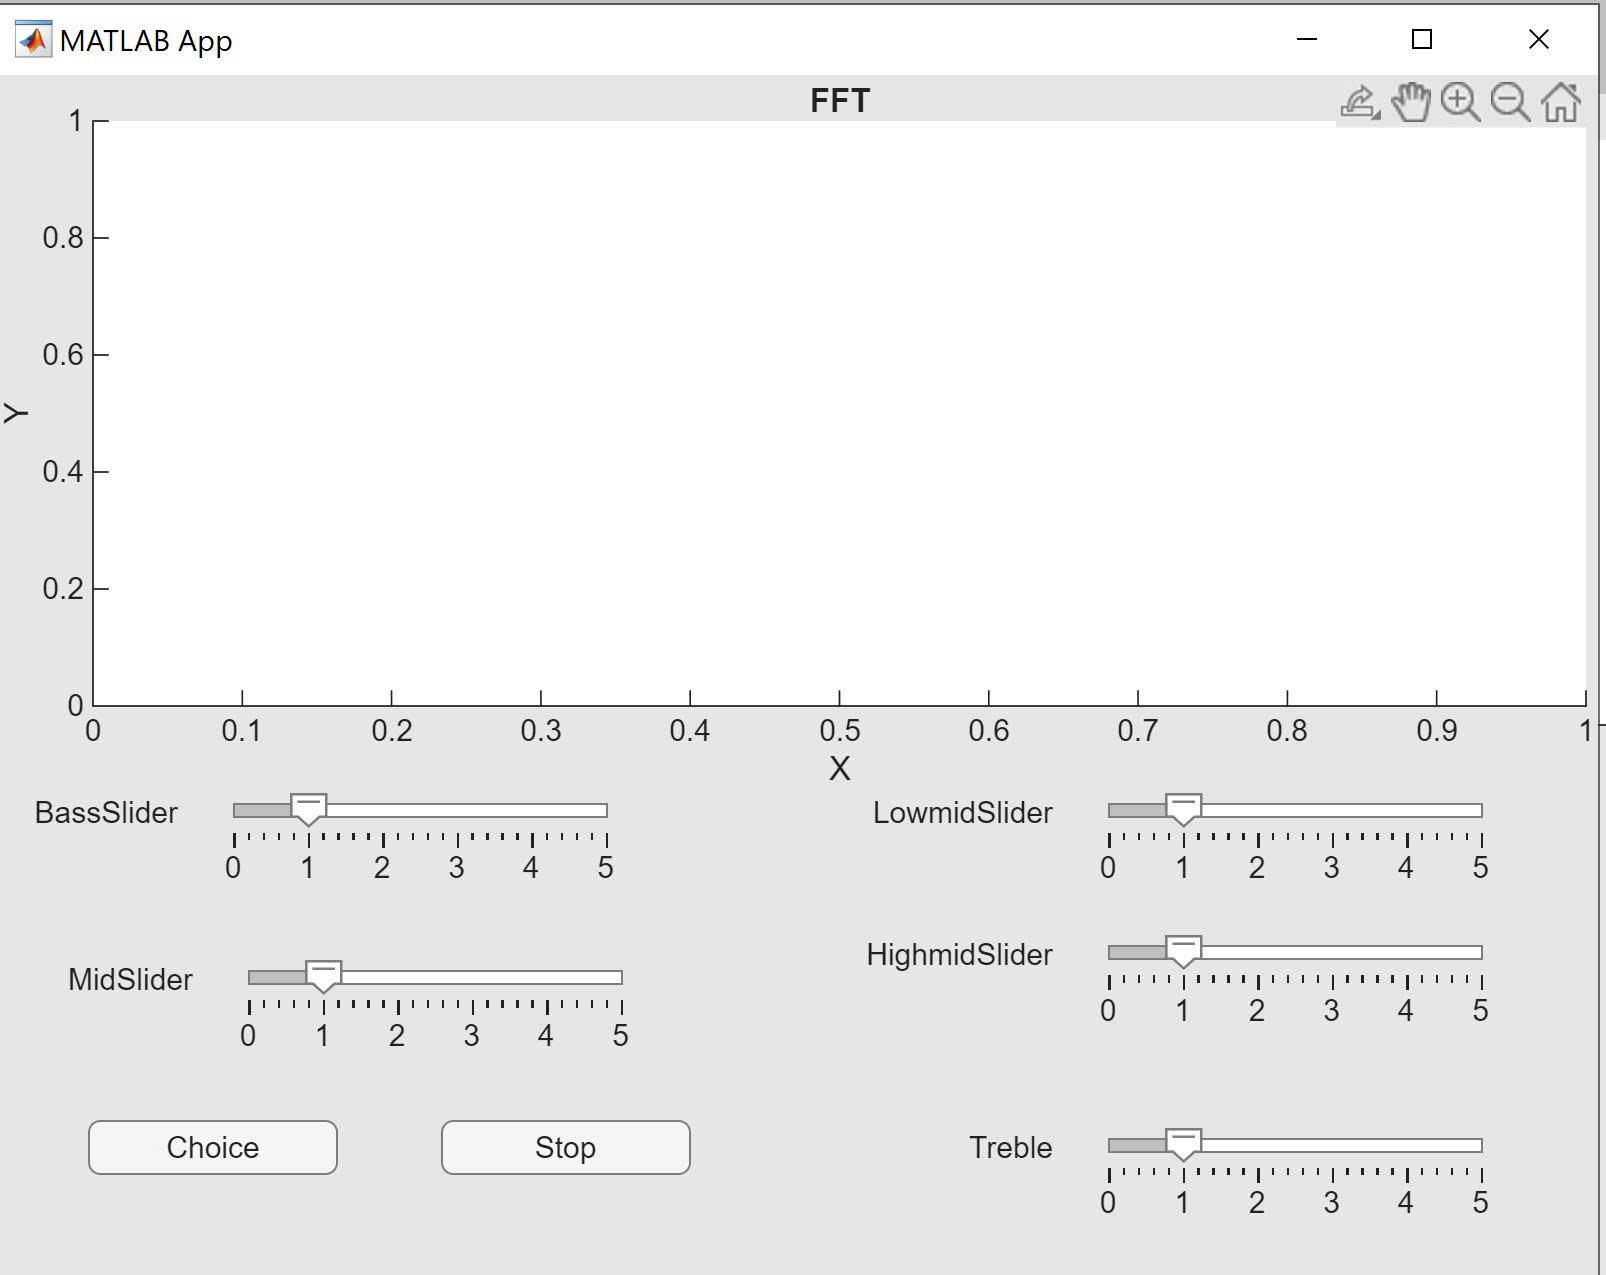
\includegraphics[width=0.9\textwidth]{interface_GUI.jpg}
    \caption{Giao diện tương tác người dùng của trạm xử lý âm thanh}
    \label{fig:gui_app}
\end{figure}
\section{Kết luận và Hướng phát triển}

\subsection{Kết quả đạt được}
Hệ thống đã hoàn thành xuất sắc các mục tiêu đề ra ban đầu về cả khía cạnh thuật toán xử lý lẫn giao diện người dùng. Cụ thể, đề tài đã đạt được những kết quả nổi bật sau:
\begin{itemize}[label=$\bullet$]
    \item \textbf{Về mặt thuật toán:} Thiết kế thành công hệ thống bộ lọc IIR Butterworth bậc 4. Việc áp dụng linh hoạt cấu trúc phân rã SOS (\texttt{zp2sos}) và kỹ thuật lọc hai chiều (\texttt{filtfilt}) đã giúp triệt tiêu hoàn toàn sai số lượng tử hóa và hiện tượng méo pha cố hữu của họ bộ lọc IIR. Qua đó, hệ thống phân tách dải tần hoạt động với độ chính xác cao, dốc cắt tần lý tưởng và bảo toàn nguyên vẹn âm thanh gốc.
    
    \item \textbf{Về mặt ứng dụng:} Xây dựng thành công trạm xử lý âm thanh (Audio Equalizer) trên nền tảng MATLAB App Designer. Giao diện người dùng được thiết kế trực quan và thân thiện, cho phép người dùng tùy chỉnh hệ số khuếch đại cho 5 dải tần số độc lập, đồng thời trực tiếp quan sát sự biến đổi phổ FFT theo thời gian thực mà không gặp hiện tượng trễ (latency) hay gián đoạn luồng phát.
\end{itemize}

\subsection{Hạn chế của hệ thống}
Mặc dù đáp ứng tốt các yêu cầu về xử lý tín hiệu, hệ thống hiện tại vẫn tồn tại một số giới hạn nhất định. Trạm xử lý hiện chỉ đang tập trung thao tác trên các luồng dữ liệu âm thanh ngoại tuyến (đọc từ các định dạng tệp \texttt{.wav}, \texttt{.mp3} có sẵn trong bộ nhớ). Hệ thống chưa hỗ trợ giao tiếp với phần cứng máy tính để thu nhận và xử lý tín hiệu truyền trực tiếp từ micro (real-time microphone streaming).

\subsection{Hướng phát triển trong tương lai}
Dựa trên những kết quả đã đạt được và các hạn chế còn tồn đọng, một số hướng sẽ được phát triển dựa trên nền của hệ thống như sau:
\begin{itemize}[label=$\bullet$]
    \item \textbf{Tích hợp luồng âm thanh thời gian thực:} Nâng cấp mã nguồn kết hợp với đối tượng \texttt{audiorecorder} trong MATLAB để hệ thống có khả năng thu, lọc và phát âm thanh từ micro theo thời gian thực với độ trễ tối thiểu.
    \item \textbf{Phát triển thiết bị phần cứng độc lập:} Thay vì giới hạn trên môi trường mô phỏng phần mềm, thuật toán lọc IIR này có thể được chuyển đổi và biên dịch sang mã C/C++ bản địa (native C code) để nhúng trực tiếp lên các kiến trúc vi điều khiển (như dòng vi điều khiển STM32F103). Việc kết hợp với các IC chuyển đổi DAC/ADC chuyên dụng trên phần cứng thực tế sẽ giúp tạo ra một thiết bị Audio Equalizer di động và hoàn chỉnh.
\end{itemize}

% ==========================================
% TÀI LIỆU THAM KHẢO
% ==========================================
\newpage
\addcontentsline{toc}{section}{Tài liệu tham khảo} 
\renewcommand{\bibname}{Tài liệu tham khảo} 
\begin{thebibliography}{99}

\bibitem{ref_NLT}
Nguyễn Linh Trung, Trần Đức Tân và Huỳnh Hữu Tuệ, \textit{Xử lý tín hiệu số}, 1st ed., 2025.

\bibitem{ref_proakis}
J. G. Proakis and D. G. Manolakis, \textit{Digital Signal Processing: Principles, Algorithms, and Applications}, 5th ed. Pearson, 2021. 

\bibitem{ref_oppenheim}
A. V. Oppenheim and R. W. Schafer, \textit{Discrete-Time Signal Processing}, 3rd ed. Pearson Education, 2014.

\bibitem{ref_dafx}
U. Zölzer, \textit{DAFX: Digital Audio Effects}, 2nd ed. John Wiley \& Sons, 2011.
\bibitem{ref_acoustics}
F. A. Everest and K. C. Pohlmann, \textit{Master Handbook of Acoustics}, 6th ed. McGraw-Hill Education, 2014.

\bibitem{ref_mathworks_filtfilt}
MathWorks, ``Zero-phase digital filtering - filtfilt,'' \textit{MATLAB \& Simulink Documentation}, 2026. [Trực tuyến].

\bibitem{ref_mathworks_zp2sos}
MathWorks, ``Zero-pole-gain to second-order sections model conversion - zp2sos,'' \textit{MATLAB \& Simulink Documentation}, 2026. [Trực tuyến]. 

\bibitem{ref_mathworks_appdesigner}
MathWorks, ``MATLAB App Designer: Build Apps with Interactive UI Components,'' \textit{MATLAB Documentation}, 2026. [Trực tuyến]. 

\end{thebibliography}


% ==========================================
% PHỤ LỤC
% ==========================================
\newpage

\clearpage 

\section*{PHỤ LỤC} 
\phantomsection
\addcontentsline{toc}{section}{Phụ lục} 

\subsection*{Mã nguồn dự án} 
\phantomsection
\addcontentsline{toc}{subsection}{Mã nguồn dự án} 

Toàn bộ mã nguồn chương trình xử lý tín hiệu (MATLAB App Designer) và tệp nguồn cấu trúc báo cáo của đề tài được lưu trữ công khai trực tuyến. Người đọc có thể truy cập tham chiếu, kiểm tra thuật toán phân tách dải tần số và chạy thử nghiệm giao diện điều khiển thông qua đường dẫn chính thức dưới đây:

\vspace{0.3cm}
\noindent Đường dẫn kho lưu trữ (GitHub Repository): \\
\url{https://github.com/24021830-tth/Audio-Equalizer-DSP}


\end{document}